%% O LaTeX é bastante modular, e utiliza pacotes para tarefas específicas
%% Todo documento tem dois blocos: preâmbulo e  documento
%% O preâmbulo contém elementos essenciais para a cofiguração da saída gerada (por exemplo, um PDF de alta qualidade)
%% Todo preâmbulo tem uma "classe de documento"
%% Neste caso, teremos um artigo, com saída em papel a4 e fonte 12 pt
\documentclass[a4paper, 12pt]{article} %definição do tipo de documento
\usepackage[a4paper, top=3cm, left=3cm, bottom=2cm, right=2cm]{geometry} % pacote para definição das margens
\usepackage{graphicx} % pacote para a inserção de gráficos
\usepackage[utf8]{inputenc} % pacote para a utilização de caracteres especiais da língua portuguesa
\usepackage[brazil]{babel} % pacote para utilização de hifenização em pt_BR

%% pacotes necessários para a fonte Arial (que deriva da fonte Helvetica)
\usepackage[T1]{fontenc}
\usepackage{helvet}
\renewcommand{\familydefault}{\sfdefault}
%%

%% O pacote showframe mostra um quadro em torno do texto, de forma que se pode verificar o posicionamento em relação às margens
%\usepackage{showframe}
\usepackage{csquotes} % pacote para facilitar citações
\usepackage{indentfirst} % pacote para indentação do primeiro parágrafo
%% Pacotes AMS
\usepackage{amsmath}
\usepackage{amstext} 
\usepackage{amssymb} 
\usepackage{caption} % pacote para controle facilitado das legendas
\usepackage{setspace} % pacote para simplificar a adição de espaços entre caracteres
\usepackage[input-decimal-markers={,},output-decimal-marker={,},]{siunitx} % pacote para utilização de unidades SI e vírgula como separador decimal
\usepackage[usenames,dvipsnames]{xcolor} % pacote para facilitar o uso de cores

%% pacotes para uso do tikz
\usepackage{tikz}
\usetikzlibrary{scopes}
\usetikzlibrary {arrows.meta}
%%

%% pacotes necessários para a bibliografia
\usepackage[
backend=biber,
style=abnt,
uniquelist=false,
sorting=nty
]{biblatex}
\addbibresource{bibliografia.bib} % arquivo com as referências bibliográficas
%% 

% definição do nome das funções trigonométricas em português
\DeclareMathOperator{\sen}{sen}
\DeclareMathOperator{\tg}{tg}
\DeclareMathOperator{\arctg}{arctg}

% Definição de cores para as tabelas com os resultados
% Para mais cores, acesse: https://www.overleaf.com/learn/latex/Using_colours_in_LaTeX
\def\comprimido{OrangeRed!30}
\def\tracionado{OliveGreen!30}

%%%%%

%% Cabeçalho do texto
\title{Um modelo de documento \LaTeX\space para a disciplina TCC I}
\author{Maurício Mauad Menegaz Filho\footnote{\texttt{email at email.com}}}

\setstretch{1.5} % configuração do espaçamento entre linhas
%% Fim do preâmbulo, início do documento propriamente.
\begin{document}
\maketitle % este comando gera o cabeçalho
%% Resumo
\begin{abstract}Este documento é um modelo \LaTeX \space configurado para seguir as prescrições da disciplina TCC I, ministrada pela Profa. Dra. Bárbara Jordani, para o curso de Bacharelado em Engenharia Civil da Uniavan. Os detalhes da configuração podem ser obtidos no material didático disponibilizado no {\tt blackboard}. Para exemplificar o uso do \LaTeX, optou-se por resolver um problema simples de análise estrutural: o cálculo dos esforços nas barras de uma treliça tipo Warren. Além da solução analítica, através do método dos nós, foi utilizada a ferramenta computacional FTool \cite{ftool}. O comparativo entre os resultados, demonstra a consistência e assertividade na aplicação dos métodos numéricos utilizados na ferramenta.
\end{abstract}

% As seções são numeradas automaticamente pelo LaTeX
\section{Introdução}

Este texto apresenta exemplos práticos na utilização do \LaTeX\space para a elaboração de um artigo acadêmico em engenharia civil. A formatação do artigo, se dá conforme a NBR 6022 \cite{nbr6022}. As referências seguem a NBR 6023 \cite{nbr6023}, e as citações são conformes a NBR 10520 \cite{nbr10520}. 
O objetivo do trabalho, é ilustrar no uso de vários elementos usuais em trabalhos acadêmicos em engenharia: equações, tabelas, figuras, referências, citações e bibliografia.

As treliças são estruturas essenciais em engenharia. Das pontes às coberturas, treliças servem como modelo prático e econômico para diversas soluções. Por exemplo, as treliças aparecem em várias seções da NBR 6118 \cite{nbr6118}, servindo como modelo estrutural para a análise de fenômenos como torção e cisalhamento em peças de concreto armado. Para este trabalho, utilizou-se uma treliça do tipo Warren simples, sem montantes entre os banzos inferior e superior, somente diagonais. 

\section{Referencial teórico}
Segundo \cite{beerjohnston}, treliças consistem em barras retas, sujeitas a duas forças, conectados por nós nas extremidades. A treliça Warren bi-apoiada é um modelo estaticamente determinado, portanto, a tarefa de encontrar os esforços nas barras tem solução analítica. 

Neste caso, pode-se utilizar tanto o método dos nós, quanto o método das seções. Pode-se ainda tirar vantagens de eventuais simetrias do problema, facilitando os cálculos. 

Por outro lado, soluções de problemas estaticamente indeterminados, requerem métodos mais sofisticados para o cálculo dos esforços. Uma introdução detalhada sobre métodos de análise estrutural, como o método dos deslocamentos, e o método da rigidez direta, encontra-se em \cite{martha}. O autor deste livro, o Dr. Luiz Martha, é o desenvolvedor do FTool. 
 
\begin{figure}[!ht]
    \centering
    \caption{Treliça Warren utilizada para a elaboração deste trabalho. A treliça vence um vão de 20 m, tem 5 m de altura, composta por nove barras, conectadas por quinze nós. O apoio A é de segundo gênero, e o apoio B é de primeiro gênero. Para o cálculo dos esforços axiais, a seção e material das barras é irrelevante.} 
    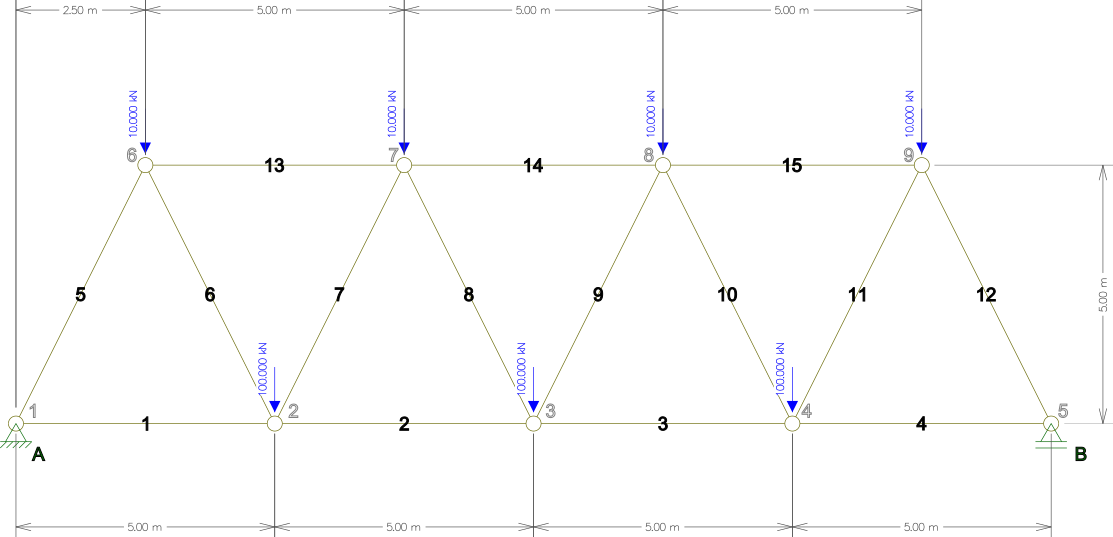
\includegraphics[width=\linewidth]{Warren-model.png}
    \caption*{Fonte: o autor.}
    \label{fig:warren-model}
\end{figure}

\begin{table}[t]
    \centering
    \caption{Coordenadas cartesianas dos nós da treliça.}
    \begin{tabular}{crr|crr|crr}
        \hline\hline
        Nó & $x\,[\unit{m}]$  & $y\,[\unit{m}]$ & Nó & $x\,[\unit{m}]$  & $y\,[\unit{m}]$ & Nó & $x\,[\unit{m}]$  & $y\,[\unit{m}]$ \\
        \hline\hline
        1 & 0,00 & 0,00 & 4 & 0,00 & 15,00 & 7 &  7,50 & 5,00 \\
        \hline
        2 & 0,00 & 5,00 & 5 & 0,00 & 20,00 & 8 & 12,50 & 5,00 \\
        \hline
        3 & 0,00 & 10,00 & 6 & 2,50 & 5,00 & 9 & 15,00 & 5,00 \\
        \hline\hline
    \end{tabular}
    \vspace{3mm}
    \caption*{Fonte: o autor.}
    \label{tab:coordenadas}
\end{table}

\section{Metodologia}\label{sec:metodologia}
A obtenção de uma solução analítica, consiste na aplicação do método dos nós, ou do método das seções. Para o problema em questão, as seguintes premissas foram adotadas:
\begin{itemize}
    \item A treliça é plana
    \item Todos as barras são conectados por pinos, e podem girar livremente no plano
    \item As barras estão sujeitas somente a esforços axiais
    \item As cargas atuam sobre os nós
    \item Em princípio, assume-se que as barras estão em sujeitas a esforços de tração, e um sinal negativo implica que a barra está em compressão
\end{itemize}
    
Os passos da solução são dados a seguir:
\begin{enumerate}
\item Verificação das condições necessárias e suficientes para a aplicação do método dos nós
\item Determinação das reações de apoio
\item Traçado do diagrama de corpo livre para cada nó
\item Cálculo das forças através da aplicação das condições de equilíbrio estático
\end{enumerate}

Em relação aos resultados numéricos obtidos pelos cálculos manuais, utilizou-se um critério normalmente adotado na solução de problemas com o uso da calculadora: limitou-se as casas decimais e três, seguindo o critério de arredondamento dado pela ABNT NBR 5891 \cite{nbr5891}. 

A solução computacional, através do FTool, não explicita qual metodologia de operação com ponto flutuante utiliza. Assumiu-se que segue o padrão \cite{1985--ieee754}.

\section{Desenvolvimento}

Para a modelagem computacional do problema, pode-se utilizar tanto as cotas na fig. (\ref{fig:warren-model}), quanto as coordenadas cartesianas da tabela (\ref{tab:coordenadas}).

\subsection{Método dos nós}
Conforme a sequência prescrita na seção (\ref{sec:metodologia}), é necessário avaliar o grau de hiperestaticidade da treliça descrita na fig. (\ref{fig:warren-model}). Segundo \cite{martha}, o grau de hiperestaticidade $g$ de uma treliça plana é dado por:
\begin{equation}
    g = \sum r + \sum m - 2\sum j \label{eq:g} 
\end{equation}
onde $r$ é o número de componentes das reações de apoio, $m$ é o número de barras
pela diferença entre o número de incógnitas do problema estático, e $j$ é o número de nós. Desta forma, os modelos estruturais podem ser classificados como:
\begin{itemize}
    \item $g < 0\,\rightarrow$ condição suficiente para o modelo ser hipostático e instável;
    \item $g = 0\,\rightarrow$ condição necessária para o modelo ser isostático e estável;
    \item $g < 0\,\rightarrow$ condição necessária para o modelo ser hiperestático e estável.
    
\end{itemize}

A treliça em análise tem três reações de apoio: $R_{A,x},\, R_{A,y}$ e $R_{B,y}$, $m = 15$, e $j = 9$. Aplicando-se a eq. (\ref{eq:g}), tem-se que:
\begin{align}
    g & = 3 + 15 - 2\times 9\\
      & = 0
\end{align} 

Desta forma, a condição necessária para uma estrutura isostática estável está satisfeita. As condições suficientes, são dadas por $g = 0$, mais as premissas adotadas para o cálculo na seção (\ref{sec:metodologia}). 

\subsubsection{Convenção de sinais}
Para os cálculos realizados neste trabalho, considera-se o plano cartesiano com o eixo $\rightarrow +x$ positivo para a direita, o eixo $\uparrow +y$ positivo para cima, o momento positivo no sentido horário $\circlearrowright +M$, esforços de tração com sinal positivo $+F$, e esforços de compressão com sinal negativo $-F$.

\subsubsection{Simetria do problema}
Posto que tanto a geometria da treliça, quanto os carregamentos são simétricos, pode-se escrever que:
\begin{align}
F_1 &= F_4 \\
F_2 &= F_3 \\
F_5 &= F_{12} \\
F_6 &= F_{11} \\
F_7 &= F_{10} \\
F_8 &= F_9 \\
F_{13} &= F_{15} 
\end{align}
o que implica que somente os esforços em oito barras precisam ser determinados. 

Como não existem esforços horizontais, as reações de apoio são iguais, ou seja $R_{A,y} = R_{B, y}$.

% definição de uma variável para facilitar a escrita do ângulo 
\def\angulodiagonais{63,435^\circ}
O ângulo entre os banzos e as diagonais vale $\arctg({2}) \approx \angulodiagonais$.

\subsubsection{Determinação das reações de apoio}

As reações de apoio são dadas pela aplicação das condições de equilíbrio:

{\noindent $\sum F_x = 0$}
\begin{equation}
    R_{A,x} = \qty{0}{kN}
\end{equation}
{\noindent $\sum F_y = 0$}
\begin{align}
      R_{A,y} + R_{B_y} &- 100 - 100 - 100 - 10 - 10 - 10 - 10 = 0\\
      R_{A,y} + R_{B_y} & = 340
\end{align}

Como $R_{A,y} = R_{B,y}$, tem-se que:
\begin{align}
    2R_{A,y} &= 340 \\
    R_{A,y} & = \qty{170}{kN} \\
    R_{B,y} & = \qty{170}{kN}
\end{align}

Também se pode obter $R_{B,y}$ através da terceira condição de equilíbrio:
{\noindent $\sum M_A = 0$}
\begin{align}
    -20R_{B,y} &+ 5\times 100 + 10\times 100 + 15\times 100 + 2,50\times 10 \\
               &+ 7,50\times10 + 12,50 \times 10 + 17,50\times 10 = 0\\
    R_{B, y}  &=\frac{1}{20}\\
    R_{B, y}  &= \qty{170}{kN}
\end{align}

\subsubsection{Nó 1}
%% Diagram de corpo livre nó 1
\begin{figure}[!ht]
    \centering
    \caption{Diagrama de corpo livre do nó 1. }
    %% DCL nó 1
    \begin{tikzpicture}[
        force+/.style={>={Stealth[length=3mm]},draw=green,fill=green},
        force-/.style={>={Stealth[length=3mm]},draw=red,fill=red},
        dot/.style = {circle, fill=black!50, minimum size=#1, inner sep=0pt, outer sep=0pt},
        dot/.default = 6pt,
    ]
    \node[dot,label=below right:Nó 1] at (0,0) {};
    % F5
    \draw[-{Stealth[length=3mm]}] (0,0) -- (1.25,2.5) node[anchor=north west]{$F_5$};
    % F13
    \draw[-{Stealth[length=3mm]}] (0,0) -- (2.5,0) node[anchor=north west]{$F_1$};
    % RAx
    \draw[force+,->] (-2,0) -- (0,0) node[anchor=south west]{};
    \node[anchor=south west] at (-2.75,-0.65) {{$R_{A,x} = \qty{0}{kN}$}};
    % Ray
    \draw[force+,->] (0,-2) -- (0,0) node[anchor=south west]{};
    \node[] at (1.85, -1.75) {{$R_{A,y} = \qty{170,000}{kN}$}};
    \end{tikzpicture}
    \caption*{Fonte: o autor}
    \label{fig:dclnó1}
\end{figure}
%%

{\noindent $\sum F_x = 0$}
\begin{align}
    &R_{A,x} + F_1 + F_5 \cos(\angulodiagonais) = 0\\
    &F_1 + F_5\times0,447 = 0\\
    &F_1 = - F_5\times0,447\label{eq:F1}
\end{align}

{\noindent $\sum F_y = 0$}
\begin{align}
    &R_{A,y} + F_5 \sen(\angulodiagonais) = 0\\
    &170,000 + F_5\times0,894 = 0\\
    &F_5 = -\frac{170,000}{0,894}\\
    &F_5 = \qty{-190,157}{kN}\label{eq:F5}
\end{align}

Substituindo-se (\ref{eq:F5}) em (\ref{eq:F1}), tem-se que:
\begin{align}    
    &F_1 + -(-190,157)\times0,447 = 0\\
    &F_1 = \qty{85,000}{kN}
\end{align}


\subsubsection{Nó 6}
%% Diagram de corpo livre do nó 6
\begin{figure}[!ht]
    \centering
    \caption{Diagrama de corpo livre do nó 6.}
    %% DCL nó 6
    \begin{tikzpicture}[
        force+/.style={>={Stealth[length=3mm]},draw=green,fill=green},
        force-/.style={>={Stealth[length=3mm]},draw=red,fill=red},
        dot/.style = {circle, fill=black!50, minimum size=#1, inner sep=0pt, outer sep=0pt},
        dot/.default = 6pt,
    ]
    \node[dot,label=above right:Nó 6] at (0,0) {};
    % F13
    \draw[-{Stealth[length=3mm]}] (0,0) -- (2.5,0) node[anchor=north west]{$F_{13}$};
    % F5
    \draw[-{Stealth[length=3mm]}] (0,0) -- (-1.25,-2.5); 
    \node[] at (-1.75,-2.85){$F_5 = \qty{-190,157}{kN}$};
    % F6
    \draw[-{Stealth[length=3mm]}] (0,0) -- (1.25,-2.5) node[anchor=north west]{$F_6$};
    % Carga 10 kN
    \draw[force-,->] (0,2) -- (0,0) node[anchor=south west]{};
    \node[] at (0.75, 2) {{$\qty{10}{kN}$}};
    \end{tikzpicture}    
    \caption*{Fonte: o autor.}
    \label{fig:dclnó6}
    \end{figure}
%%
{\noindent $\sum F_x = 0$}
\begin{align}
    -&F_5\cos(\angulodiagonais) + F_6\cos(\angulodiagonais) + F_{13} = 0\\
    -&F_5\times0,447 + F_6\times0,447 + F_{13}= 0\\
    &84,240 + F_6\times0,447 + F_{13}= 0 \label{eq:nó6x}
\end{align}

{\noindent $\sum F_y = 0$}
\begin{align}
    -&10 -F_5\sen(\angulodiagonais) - F_6\sen(\angulodiagonais) = 0\\
    -&10 + 190,157\times0,894  - F_6\times0,894 = 0 \\
     &F_6 = \frac{160,000}{0,894} \\
     &F_6 = \qty{178,971}{kN} \label{eq:F6}
\end{align}

Substituindo-se (\ref{eq:F6}) em (\ref{eq:nó6x}), tem-se que:
\begin{align}
    &84,240 + 178,971\times0,894 + F_{13} = 0\\
    &F_{13} = -\qty{164,240}{kN}
\end{align}

\subsubsection{Nó 2}
%% Diagrama de corpo livre do nó 2
\begin{figure}[!ht]
    \centering
    \caption{Diagrama de corpo livre do nó 2.}
    %% DCL nó 2
    \begin{tikzpicture}[
        force+/.style={>={Stealth[length=3mm]},draw=green,fill=green},
        force-/.style={>={Stealth[length=3mm]},draw=red,fill=red},
        dot/.style = {circle, fill=black!50, minimum size=#1,inner sep=0pt, outer sep=0pt},
        dot/.default = 6pt,
    ]
    \node[dot,label=below right:Nó 2] at (0,0) {};
    % F1
    \draw[-{Stealth[length=3mm]}] (0,0) -- (-2.5,0) node[anchor=north east]{$F_{1} = \qty{85,000}{kN}$};
    % F2
    \draw[-{Stealth[length=3mm]}] (0,0) -- (2.5,0) node[anchor=north west]{$F_{2}$};
    % F6
    \draw[-{Stealth[length=3mm]}] (0,0) -- (-1.25,2.5) node[]{};
    \node[] at (-2.5, 2.75) {$F_6 = \qty{178,971}{kN}$};
    % F7
    \draw[-{Stealth[length=3mm]}] (0,0) -- (1.25,2.5) node[anchor=north west]{$F_7$};
    % Carga 100 kN
    \draw[force-,->] (0,3.5) -- (0,0) node[anchor=south west]{};
    \node[] at (0.75, 3.5) {{$\qty{100}{kN}$}};
    \end{tikzpicture}
    \caption*{Fonte: o autor.}
    \label{fig:dclnó2}
    \end{figure}
%%
{\noindent $\sum F_x = 0$}
\begin{align}
    -&F_1 + F_2 -F_6\cos(\angulodiagonais) + F_7\cos(\angulodiagonais) = 0\\
    -&165,000 + F_2 + F_7\times0,447 = 0\label{eq:nó2x}
\end{align}

{\noindent $\sum F_y = 0$}
\begin{align}
    -&100 + F_6\sen(\angulodiagonais) + F_7\sen(\angulodiagonais) = 0\\
    -&100 + 160,000 + F_7\times0,894 = 0\\
    &F_7 = -\frac{60,000}{0,894}\\
    &F_7 = -\qty{67,114}{kN} \label{eq:F7}
\end{align}
Substituindo-se (\ref{eq:F7}) em (\ref{eq:nó2x}), tem-se que:
\begin{align}
    -&165,000 + F_2 -67,114\times0,447 = 0 \\
    -&165,000 + F_2 -30,000 = 0 \\
     &F_2 = \qty{195,000}{kN} \label{eq:F2}
\end{align}

\subsubsection{Nó 7}
%% Diagrama de corpo livre do nó 7
\begin{figure}[!ht]
    \centering
    \caption{Diagrama de corpo livre do nó 7.}
    %% DCL nó 7
    \begin{tikzpicture}[
        force+/.style={>={Stealth[length=3mm]},draw=green,fill=green},
        force-/.style={>={Stealth[length=3mm]},draw=red,fill=red},
        dot/.style = {circle, fill=black!50, minimum size=#1,
              inner sep=0pt, outer sep=0pt},
        dot/.default = 6pt,
    ]
    \node[dot,label=below right:Nó 7] at (0,0) {};
    % F13
    \draw[-{Stealth[length=3mm]}] (0,0) -- (-2.5,0) node[anchor=north east]{$F_{13} = \qty{-164,240}{kN}$};
    % F14
    \draw[-{Stealth[length=3mm]}] (0,0) -- (2.5,0) node[anchor=north west]{$F_{14}$};
    % F7
    \draw[-{Stealth[length=3mm]}] (0,0) -- (-1.25,-2.5) node[]{};
    \node[] at (-2.5, -2.75) {$F_7 = \qty{-67,114}{kN}$};
    % F8
    \draw[-{Stealth[length=3mm]}] (0,0) -- (1.25,-2.5) node[anchor=north west]{$F_8$};
    % Carga 10 kN
    \draw[force-,->] (0,2) -- (0,0) node[anchor=south west]{};
    \node[] at (0.75, 2) {{$\qty{10}{kN}$}};
    \end{tikzpicture}
    \caption*{Fonte: o autor.}
    \label{fig:dclnó7}
\end{figure}
%% 

{\noindent $\sum F_x = 0$}
\begin{align}
    -&F_7\cos(\angulodiagonais) + F_8\cos(\angulodiagonais) - F_{13}  + F_{14}= 0\\
    &67,114\times0,447 + F_8\times0,447 + 164,240 + F_{14} = 0 \\
    &F_{14} + F_8\times0,447 + 231,354 = 0 \label{eq:nó7x}
\end{align}

{\noindent $\sum F_y = 0$}
\begin{align}
    -&10 - F_7\sen(\angulodiagonais) - F_8\sen(\angulodiagonais) = 0\\
    -&10 + 67,114\times0,894 - F_8\times0,894 = 0\\
    &F_8 = -\frac{50,000}{0,894} \\
    &F_8 = -\qty{55,928}{kN} \label{eq:F8}
\end{align}

Substituindo-se (\ref{eq:F8}) em (\ref{eq:nó7x}), tem-se que:
\begin{align}
     &F_{14} + 55,928\times 0,447 + 194,240 = 0 \\
     &F_{14} = \qty{219,240}{kN} \label{eq:F14}
\end{align}


\begin{table}[!ht]
    \centering
    \caption{Resultados obtidos pelo método dos nós para os esforços axiais nas barras da treliça.}
    \begin{tabular}{cr cr cr cr}
        \hline\hline
        Barra & F $[\unit{kN}]$ & Barra & F $[\unit{kN}]$ & Barra & F $[\unit{kN}]$ & Barra & F $[\unit{kN}]$\\
        \hline\hline
        1 & \colorbox{\tracionado}{85,000}  & 5 & \colorbox{\comprimido}{-190,157}  & 9  &  \colorbox{\tracionado}{55,902} & 13 & \colorbox{\comprimido}{-165,000} \\
        \hline
        2 & \colorbox{\tracionado}{195,000} & 6 &  \colorbox{\tracionado}{178,971}  & 10 & \colorbox{\comprimido}{-67,082} & 14 & \colorbox{\comprimido}{-220,000} \\
        \hline
        3 & \colorbox{\tracionado}{195,000} & 7 &  \colorbox{\comprimido}{-67,114}  & 11 & \colorbox{\tracionado}{178,855} & 15 & \colorbox{\comprimido}{-165,000} \\
        \hline
        4 & \colorbox{\tracionado}{85,000}  & 8 &  \colorbox{\tracionado}{55,928}   & 12 &\colorbox{\comprimido}{-190,066} &   &   \\
        \hline\hline
    \end{tabular}
    \vspace{3mm}
    \caption*{Fonte: o autor.}
    \label{tab:esforços_nós}
\end{table}

\subsection{Solução utilizando o FTool}

O FTool é uma ferramenta simples, e consagrada para análise de estruturas planas. Embora muito utilizado no meio acadêmico, o programa pode também ser utilizado como suporte no cálculo das reações e esforços de diversas estruturas que podem ser decompostas em pórticos planos. O FTool tem uma versão gratuita, totalmente funcional, e uma versão paga, com capacidades adicionais avançadas. 

A figura (\ref{fig:warren-ftool}) traz a solução para os esforços nas barras da treliça Warren proposta neste trabalho. O arquivo FTool utilizado para a simulação, pode ser obtido no repositório GitHub em \cite{maumenegaz}.

\begin{figure}[!ht]
    \centering
    \caption{Solução obtida pelo FTool para a treliça Warren. As barras comprimidas são mostradas em vermelho, enquanto as barras tracionadas são mostradas em verde. Os diagramas de força normal e as reações também são mostrados no diagrama.} 
    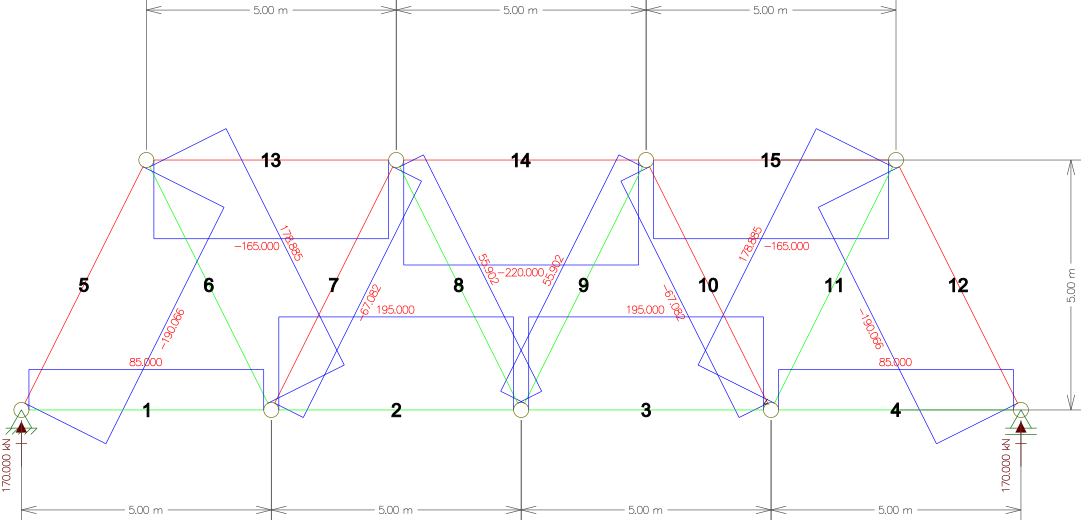
\includegraphics[width=\linewidth]{Warren-model-FTool-Solution.png}
    \caption*{Fonte: o autor.}
    \label{fig:warren-ftool}
\end{figure}


\begin{table}[!ht]
    \centering
    \caption{Resultados obtidos pelo FTool para os esforços axiais nas barras da treliça.  }
    \begin{tabular}{cr cr cr cr}
        \hline\hline
        Barra & F $[\unit{kN}]$ & Barra & F $[\unit{kN}]$ & Barra & F $[\unit{kN}]$ & Barra & F $[\unit{kN}]$\\
        \hline\hline
        1 & \colorbox{\tracionado}{85,000}  & 5 & \colorbox{\comprimido}{-190,066}  & 9  &  \colorbox{\tracionado}{55,902} & 13 & \colorbox{\comprimido}{-165,000} \\
        \hline
        2 & \colorbox{\tracionado}{195,000} & 6 &  \colorbox{\tracionado}{178,855}  & 10 & \colorbox{\comprimido}{-67,082} & 14 & \colorbox{\comprimido}{-220,000} \\
        \hline
        3 & \colorbox{\tracionado}{195,000} & 7 &  \colorbox{\comprimido}{-67,082}  & 11 & \colorbox{\tracionado}{178,855} & 15 & \colorbox{\comprimido}{-165,000} \\
        \hline
        4 & \colorbox{\tracionado}{85,000}  & 8 &  \colorbox{\tracionado}{55,902}   & 12 &\colorbox{\comprimido}{-190,066} &   &   \\
        \hline\hline
    \end{tabular}
    \vspace{3mm}
    \caption*{Fonte: o autor.}
    \label{tab:esforços_ftool}
\end{table}


\subsection{Resultados}

Combinando-se os valores obtidos para os esforços, conforme as tabelas (\ref{tab:esforços_nós}) e (\ref{tab:esforços_ftool}), pode-se construir uma tabela comparativa.

% Tabela gera a partir de uma planilha Google Docs através do site https://www.tablesgenerator.com/
\begin{table}[!ht]
    \centering
    \caption{Tabela comparativa com os dados obtidos pelas duas metodologias. }
    \begin{tabular}{crrrr}
        \hline\hline
        Barra & M. nós [\unit{kN}] & FTool [\unit{kN}] & Dif. [\unit{kN}] & Erro 
        [\%] \\
        \hline\hline
        1     & 85,000      & 85,000     & 0,000          & 0,00     \\
        \hline
        2     & 195,000     & 195,000    & 0,000          & 0,00     \\
        \hline
        3     & 195,000     & 195,000    & 0,000          & 0,00     \\
        \hline
        4     & 85,000      & 85,000     & 0,000          & 0,00     \\
        \hline
        5     & -190,157    & -190,066   & -0,091         & 0,05     \\
        \hline
        6     & 178,971     & 178,855    & 0,116          & 0,06     \\
        \hline
        7     & -67,114     & -67,082    & -0,032         & 0,05     \\
        \hline
        8     & 55,928      & 55,902     & 0,026          & 0,05     \\
        \hline
        9     & 55,928      & 55,902     & 0,026          & 0,05     \\
        \hline
        10    & -67,114     & -67,082    & -0,032         & 0,05     \\
        \hline
        11    & 178,971     & 178,855    & 0,116          & 0,06     \\
        \hline
        12    & -190,157    & -190,066   & -0,091         & 0,05     \\
        \hline
        13    & -164,240    & -165,000   & 0,760          & -0,46    \\
        \hline
        14    & -219,240    & -220,000   & 0,760          & -0,35    \\
        \hline
        15    & -164,240    & -165,000   & 0,760          & -0,46    \\
        \hline\hline
    \end{tabular}
    \caption*{Fonte: o autor.}    
    \label{tab:comparativo}
\end{table}

Uma análise da tabela (\ref{tab:comparativo}), revela uma diferença máxima de pouco menos que 0,5\% nos resultados dos esforços comparados.

Tanto o método de solução numérica, quanto a forma de representação digital dos números de ponto flutuante, induzem erros na solução de problemas computacionais, podendo eventualmente comprometer o significado dos resultados \cite{Roy1971}. 
 
\section{Conclusão}

Demonstrou-se que os resultados analítico e numérico concordam entre si, tanto atentando para os erros induzidos pelo arredondamento numérico utilizado nos cálculos manuais, quanto validando a implementação da ferramenta computacional utilizada como consistente. Do ponto de vista numérico, não há solução exata para o problema, já que os cálculos que envolvem geometria, invariavelmente envolvem funções transcendentais, que invariavelmente terão valores de saída arredondados, a despeito da precisão de ponto flutuante utilizada. Estes achados, corroboram para o fato que a engenharia, trata-se de uma disciplina aplicada, e, portanto, manifestamente experimental. Uma simples treliça, mesmo com solução analítica, expõe diversas limitações das ferramentas e métodos de cálculo empregados em engenharia. Com tudo isso, é importante que o engenheiro compreenda estes limites, e consiga utilizá-los a seu favor enquanto projeta e assume responsabilidades sobre os projetos. 

Estas comparações numéricas, além de possuírem valor didático, servem para verificação da precisão e acurácia das soluções oferecidas por programas computacionais. Este tipo de atividade é essencial para o entendimento dos métodos, das ferramentas, e especialmente a compreensão das eventuais limitações do cálculo numérico, seja executado em computadores digitais, ou manualmente em calculadoras manuais muito mais limitadas computacionalmente.

Há diversas extensões possíveis para este trabalho. Uma extensão simples, consiste na aplicação do método da rigidez direta para o cálculo dos esforços. Pode-se escrever um programa de computador em uma linguagem acessível e moderna, como python, para verificar a qualidade comparativa dos resultados. 

%% Bibliografia
\printbibliography
\end{document}
